\errorcontextlines32
\documentclass[twoside]{report}
\usepackage[chatter]{rotating}
\usepackage{fancyvrb}
\makeatletter
\newsavebox{\@display}
\newcommand\@@Display[1]{%
 \sbox\@display{%
  \begin{minipage}[b]{.45\textwidth}%
  #1\end{minipage}%
 }\raisebox{\depth}{\usebox{\@display}}%
}

\newcommand\@@VDisplay[1]{%
 \sbox\@display{%
   \begin{minipage}[b]{.45\textwidth}%
     \BVerbatimInput[fontsize=\small]{#1}%
   \end{minipage}}%
   \usebox{\@display}%
}
\newcommand\SideBySide[2]{%
\bgroup\def\baselinestretch{1}%
 \trivlist\item[]%
 \leavevmode
 \makebox[\textwidth][l]{\@@Display{#1}\hspace{1em}%
                             \@@VDisplay{#2}}%
 \endtrivlist
 \egroup
}
\newcommand\BeginExample{%
  \nobreak
  \VerbatimEnvironment
  \catcode`\<=12
  \begin{VerbatimOut}{\jobname.ex}%
}
\newcommand{\EndExample}{\end{VerbatimOut}}

\newenvironment{example}
 {\nobreak
  \VerbatimEnvironment
  \catcode`\<=12
  \begin{VerbatimOut}{\jobname.ex}%
 }
 {\end{VerbatimOut}
  \SideBySide {\input{\jobname.ex}}%
                {\jobname.ex}}
\makeatother
%-------------------------------------------------------
\def\degrees{{\small$^{\mathrm{o}}$}}
%-------------------------------------------------------

\begin{document}

\title{Test of `rotating' package}
\author{Sebastian Rahtz and Leonor Barroca\thanks{Now maintained as part of the \LaTeX\ graphics bundle.}}
\date{November 19th 1994\thanks{Updated for graphics bundle 2016/05/22}}
\maketitle

`Rotating' provides a generalised rotation environment, where the text
will be rotated (anti-clockwise) by the number of degrees specified as
a parameter to the environment, but no special arrangement is made to
find space for the result.

\begin{example}
Start here
\begin{rotate}{-56}
Save whales
\end{rotate}
End here
\end{example}

A complete example of rotating text without leaving space
would the `Save the whale' text
written at 10 degree intervals round the compass. We use
`rlap' to ensure that all the texts are printed at the same point.
Just to show that \TeX\ can handle PostScript muckings-about
properly\ldots
\begin{example} 
\newcount\wang
\newsavebox{\wangtext}
\newdimen\wangspace
\def\wheel#1{\savebox{\wangtext}{#1}%
\wangspace\wd\wangtext
\advance\wangspace by 1cm%
\centerline{%
\rule{0pt}{\wangspace}%
\rule[-\wangspace]{0pt}{\wangspace}%
\wang=-180\loop\ifnum\wang<180
\rlap{\begin{rotate}{\the\wang}%
\rule{1cm}{0pt}#1\end{rotate}}%
\advance\wang by 10\repeat}}
\wheel{Save the whale}
\end{example}

If the user
desires \LaTeX\ to leave space for the rotated box, then `turn' is used:
\begin{example}
 Start here \begin{turn}{56}%
   Save the whale
  \end{turn} end here
\end{example}
The environment `Sideways' is a  special case, setting the rotation to $-90$,
and leaving the correct space for the rotated box. 
\begin{example}
Start here
\begin{sideways}%
Save the whale
\end{sideways}
End here
\end{example}

If you deal with whole paragraphs of text, you realize that \TeX\
boxes are not as simple as they sometimes look: they have a height
{\em and} a depth. So when you rotate, you rotate about the point on
the left-hand edge of the box that meets the baseline. The results can
be unexpected, as shown in the full set of  paragraph rotations in
Figures \ref{angles1} and \ref{angles2}. If you really want to turn a
paragraph so that it appears to rotate about the {\em real} bottom of
the \TeX\ box,
you have to adjust the box in the normal \LaTeX\ way:
\begin{example}
\newsavebox{\foo}
\savebox{\foo}{\parbox{1in}{Save 
the whales Save the whale 
Save the whale 
Save the whale}}%
Start
\begin{turn}{45}\usebox{\foo}\end{turn}
End
\end{example}
\begin{example}
\savebox{\foo}{\parbox[b]{1in}{Save 
the whales Save the whale 
Save the whale 
Save the whale}}%
Start
\begin{turn}{45}\usebox{\foo}\end{turn}
End
\end{example}

\def\testrot#1{%
\savebox{\foo}{\parbox{1in}{Save 
the whales Save the whale Save the whale Save the whale}}%
\framebox{---\begin{turn}{#1}\framebox{\usebox{\foo}}\end{turn}---}}%

\begin{figure*}
\begin{tabular}{|c|c|c|}
\hline
\testrot{0} &\testrot{-40}&\testrot{-80}\\
0\degrees & -40\degrees & -80\degrees \\
\hline
\testrot{-120}&\testrot{-160}&\testrot{-200}\\
120\degrees & -160\degrees & -200\degrees \\
\hline
\testrot{-240}&\testrot{-280}&\testrot{-320}\\
-240\degrees & -280\degrees & -320\degrees \\
\hline
\end{tabular}
\caption{Rotation of paragraphs between 0 and -320 degrees \label{angles1}}
\end{figure*}

\begin{figure*}
\begin{tabular}{|c|c|c|}
\hline
\testrot{-180} &\testrot{40}&\testrot{80}\\
-180\degrees & 40\degrees & 80\degrees \\
\hline
\testrot{120}&\testrot{160}&\testrot{200}\\
120\degrees & 160\degrees & 200\degrees \\
\hline
\testrot{240}&\testrot{280}&\testrot{320}\\
240\degrees & 280\degrees & 320\degrees \\
\hline
\end{tabular}
\caption{Rotation of paragraphs between 0 and 320 degrees\label{angles2}}
\end{figure*}


We can set tabular material in this way; at the same time, we
demonstrate that the rotation can be nested:
\begin{example}
\begin{sideways}
\rule{1in}{0pt}
\begin{tabular}{|lr|}
\em Word & \begin{rotate}{90}%
Occurrences\end{rotate}
\\
\hline
hello & 33\\
goodbye & 34\\
\hline
\end{tabular}
\end{sideways}
\end{example}

\begin{example}
\begin{quote}
\rule{0pt}{1.5in}\begin{tabular}{rrr}
\begin{rotate}{45}Column 1\end{rotate}&
\begin{rotate}{45}Column 2\end{rotate}&
\begin{rotate}{45}Column 3\end{rotate}\\
\hline
1& 2& 3\\
4& 5& 6\\
7& 8& 9\\
\hline
\end{tabular}
\end{quote}
\end{example}

\begin{example}
\begin{quote}
\begin{tabular}{rrr}
\begin{turn}{45}Column 1\end{turn}&
\begin{turn}{45}Column 2\end{turn}&
\begin{turn}{45}Column 3\end{turn}\\
\hline
1& 2& 3\\
4& 5& 6\\
7& 8& 9\\
\hline
\end{tabular}
\end{quote}
\end{example}

\begin{example}
\begin{quote}
\rule{0pt}{1.5in}\begin{tabular}{rrr}
\begin{rotate}{45}Column 1\end{rotate}
\rule{.5cm}{0pt}&
\begin{rotate}{45}Column 2\end{rotate}
\rule{.5cm}{0pt}&
\begin{rotate}{45}Column 3\end{rotate}
\rule{.5cm}{0pt}\\
\hline
1& 2& 3\\
4& 5& 6\\
7& 8& 9\\
\hline
\end{tabular}
\end{quote}
\end{example}

\begin{example}
\begin{sideways}
\begin{tabular}{|l|c|c|c|c|c|p{1in}|}
\hline
&&\multicolumn{4}{c}{NUMBER OF SITES}\vline &ACCEPT or\\
\cline{3-6} &STUDY AREA&&\multicolumn{3}{c}{%
IN BOUNDARY ZONE}\vline&REJECT\\
\cline{4-6}&&&&\multicolumn{2}{c}{EXPECTED}
\vline&NULL\\
\cline{5-6}&&TOT&OBS&FROM&TO&HYPOTH\\
\cline{2-7}
&FULL SAMPLE&41&31&10.3&27.0&REJECT\\
&SAMPLE AREA 1&23&16&4.3&16.7&ACCEPT\\
&SAMPLE AREA 2&18&15&2.8&13.7&REJECT\\
&RUSHEN&13&9&1.2&10.4&ACCEPT\\
&ARBORY&10&7&0.6&8.8&ACCEPT\\
&MAROWN&10&8&0.4&8.6&ACCEPT\\
\rule{0.5cm}{0pt}
\begin{rotate}{90}PRIMARY UNITS%
\end{rotate}\rule{0.5cm}{0pt}
&SANTON&8&7&0.0&7.3&ACCEPT\\
\hline
\end{tabular}
\end{sideways}
\end{example}

If you are interested in setting rotated material in tables or
figures, this presents no problem. Figure \ref{fig1} shows how
PostScript files which are being incorporated using can be
rotated at will, while Figure \ref{fig2} shows, in contrast, how
`includegraphics' itself handles rotation. It is also possible to rotate the
whole of the figure environment, including caption, 
by using the `sidewaysfigure' ands `sidewaystable' environments
in place of `figure' and `table'. 

Sideways figures and tables always take up the whole page. They can be
rotated so that the bottom ot the figures is on the left or the right;
the default is to always turn to the right. If the `twoside' option
has been given to the main document class, this package then starts
rotating sideways figures according to the page number (this requires
two passes through \LaTeX{} at least). If you want the `twoside'
option, but want the figures always in one direction, use the
`figuresright' or `riguresleft' options to `rotating'.

The code used to produce figures
\ref{rotfloat1}--\ref{rotfloat4} is as follows:
\begin{description}

\item[Figure \ref{rotfloat1}]
{\small\begin{verbatim}
\begin{sidewaystable}
\centering
\caption{This is a narrow  table, which should be centred vertically
on the final page.\label{rotfloat1}}
  \begin{tabular}{|ll|}
\hline
    a & b \\
    c & d \\
    e & f \\
    g & h \\
    i & j \\
\hline
  \end{tabular}
\end{sidewaystable}
\end{verbatim}
}

\item[Figure \ref{rotfloat2}]
{\scriptsize\begin{verbatim}
\begin{sidewaystable}
\centering
\begin{tabular}{|llllllllp{1in}lp{1in}|}
\hline
Context   &Length   &Breadth/   &Depth   &Profile   &Pottery   &Flint   &Animal   &Stone   &Other    &C14 Dates \\
  &         &Diameter   &        &          &          &        & 
Bones&&&\\
\hline
&&&&&&&&&&\\
\multicolumn{10}{|l}{\bf Grooved Ware}&\\
784       &---        &0.9m       &0.18m   &Sloping U &P1       &$\times$46  &  $\times$8      &&       $\times$2 bone&  2150$\pm$ 100 BC\\
785       &---        &1.00m      &0.12    &Sloping U &P2--4    &$\times$23  &  $\times$21     & Hammerstone &---&---\\
962       &---        &1.37m      &0.20m   &Sloping U &P5--6    &$\times$48  &  $\times$57*    & ---&     ---&1990 $\pm$ 80 BC (Layer 4) 1870 $\pm$90 BC (Layer 1)\\
983       &0.83m      &0.73m      &0.25m   &Stepped U &---      &$\times$18  &  $\times$8      & ---& Fired clay&---\\
&&&&&&&&&&\\
\multicolumn{10}{|l}{\bf Beaker}&\\
552       &---        &0.68m      &0.12m   &Saucer    &P7--14   &---           & ---       & ---       &---        &---\\
790       &---        &0.60m      &0.25m   &U         &P15      &$\times$12    & ---       & Quartzite-lump&---    &---\\
794       &2.89m      &0.75m      &0.25m   &Irreg.    &P16      &$\times$3     & ---       & ---       &---        &---\\
\hline
\end{tabular}
 
\caption[Grooved Ware and Beaker Features, their Finds and
Radiocarbon Dates]{Grooved Ware and Beaker Features, their
Finds and Radiocarbon Dates; For a breakdown of the Pottery
Assemblages see Tables I and III; for
the Flints see Tables II and IV; for the
Animal Bones see Table V.}\label{rotfloat2}
\end{sidewaystable}
\end{verbatim}
}

\item[Figure \ref{rotfloat3}]
{\small\begin{verbatim}
\begin{table}
\centering
\rotcaption{Minimum number of individuals; effect of rotating table
and caption separately}\label{rotfloat3}%
\begin{sideways}
\begin{tabular}[b]{cccccccccp{1cm}}
\hline
Phase&Total&Cattle&Sheep&Pig&Red Deer&Horse&Dog&Goat&Other\\
\hline
&1121&54&12&32&1&1&1&1&1 polecat\\
3&8255&58&6&35&1&1&1&1&1 roe deer, 1 hare, 1 cat, 1 otter\\
4&543&45&6&45&4&1&1&---&---\\
\hline
&9919&157&24&112&6&3&3&2&5\\
\hline
\end{tabular}
\end{sideways}
\end{table}
\end{verbatim}
}

\item[Figure \ref{rotfloat4}]
{\small\begin{verbatim}
\begin{sidewaysfigure}
  \centering
  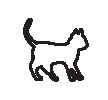
\includegraphics[width=.8\textheight,height=.4\textwidth]{cat}
\caption{A pathetically squashed rotated pussycat}\label{rotfloat4}
\end{sidewaysfigure}
\end{verbatim}
}
\end{description}

\begin{figure}
\begin{example}
---\begin{turn}{156}
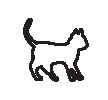
\includegraphics[width=1in]{cat}
\end{turn}---
\end{example}

\begin{example}
---\begin{sideways}
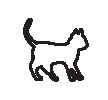
\includegraphics[width=1in]{cat}
\end{sideways}---
\end{example}

\begin{example}
---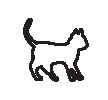
\includegraphics[width=1in]{cat}---
\end{example}
\caption{A normal, and sideways, pictures within a figure\label{fig1}}
\end{figure}

\begin{figure}
\begin{example}
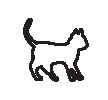
\includegraphics[width=1in,%
angle=-56]{cat}
\end{example}

\caption{Figures rotated with `includegraphics'\label{fig2}}
\end{figure}
\begin{sidewaystable}
\centering
\caption{This is a narrow  table, which should be centred vertically
on the final page.\label{rotfloat1}}
  \begin{tabular}{|ll|}
\hline
    a & b \\
    c & d \\
    e & f \\
    g & h \\
    i & j \\
\hline
  \end{tabular}
\end{sidewaystable}



\begin{sidewaystable}
\centering
\begin{tabular}{|llllllllp{1in}lp{1in}|}
\hline
Context   &Length   &Breadth/   &Depth   &Profile   &Pottery   &Flint   &Animal   &Stone   &Other    &C14 Dates \\
  &         &Diameter   &        &          &          &        & 
Bones&&&\\
\hline
&&&&&&&&&&\\
\multicolumn{10}{|l}{\bf Grooved Ware}&\\
784       &---        &0.9m       &0.18m   &Sloping U &P1       &$\times$46  &  $\times$8      &&       $\times$2 bone&  2150$\pm$ 100 BC\\
785       &---        &1.00m      &0.12    &Sloping U &P2--4    &$\times$23  &  $\times$21     & Hammerstone &---&---\\
962       &---        &1.37m      &0.20m   &Sloping U &P5--6    &$\times$48  &  $\times$57*    & ---&     ---&1990 $\pm$ 80 BC (Layer 4) 1870 $\pm$90 BC (Layer 1)\\
983       &0.83m      &0.73m      &0.25m   &Stepped U &---      &$\times$18  &  $\times$8      & ---& Fired clay&---\\
&&&&&&&&&&\\
\multicolumn{10}{|l}{\bf Beaker}&\\
552       &---        &0.68m      &0.12m   &Saucer    &P7--14   &---           & ---       & ---       &---        &---\\
790       &---        &0.60m      &0.25m   &U         &P15      &$\times$12    & ---       & Quartzite-lump&---    &---\\
794       &2.89m      &0.75m      &0.25m   &Irreg.    &P16      &$\times$3     & ---       & ---       &---        &---\\
\hline
\end{tabular}
 
\caption[Grooved Ware and Beaker Features, their Finds and
Radiocarbon Dates]{Grooved Ware and Beaker Features, their
Finds and Radiocarbon Dates; For a breakdown of the Pottery
Assemblages see Tables I and III; for
the Flints see Tables II and IV; for the
Animal Bones see Table V.}\label{rotfloat2}
\end{sidewaystable}

\begin{table}
\centering
\hbox{
\rotcaption{Minimum number of individuals; effect of rotating table
and caption separately}\label{rotfloat3}%
\begin{sideways}
\begin{tabular}[t]{cccccccccp{1cm}}
\hline
Phase&Total&Cattle&Sheep&Pig&Red Deer&Horse&Dog&Goat&Other\\
\hline
&1121&54&12&32&1&1&1&1&1 polecat\\
3&8255&58&6&35&1&1&1&1&1 roe deer, 1 hare, 1 cat, 1 otter\\
4&543&45&6&45&4&1&1&---&---\\
\hline
&9919&157&24&112&6&3&3&2&5\\
\hline
\end{tabular}
\end{sideways}
}
\end{table}


\begin{sidewaysfigure}
  \centerline{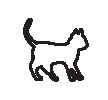
\includegraphics[width=.8\textheight,height=.4\textwidth]{cat}}
\caption{A pathetically squashed rotated pussycat (1)}
\end{sidewaysfigure}

\begin{sidewaysfigure}
  \centerline{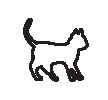
\includegraphics[width=.8\textheight,height=.4\textwidth]{cat}}
\caption{A pathetically squashed rotated pussycat (2)}
\end{sidewaysfigure}

\begin{sidewaysfigure}
  \centerline{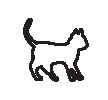
\includegraphics[width=.8\textheight,height=.4\textwidth]{cat}}
\caption{A pathetically squashed rotated pussycat (3)}
\end{sidewaysfigure}

\begin{sidewaysfigure}
  \centerline{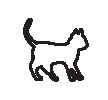
\includegraphics[width=.8\textheight,height=.4\textwidth]{cat}}
\caption{A pathetically squashed rotated pussycat (4)}
\end{sidewaysfigure}

\begin{sidewaysfigure}
  \centerline{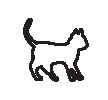
\includegraphics[width=.8\textheight,height=.4\textwidth]{cat}}
\caption{A pathetically squashed rotated pussycat}\label{rotfloat4}
\end{sidewaysfigure}

\end{document}
